\chapter{Translations}
In een ideale wereld spreekt iedereen dezelfde taal, maar zover zijn we helaas nog niet. Daarom zal je als vaak meerdere talen moeten ondersteunen in je software. In dit hoofdstuk maak je een eenvoudige translation manager. 

\begin{note}
Voor een niet al te uitgebreid programma met enkel korte zinnen is deze aanpak zeker geschikt. Wanneer je een programma met duizenden zinnen of volledige alinea's tekst maakt, dan heb je meer geavanceerde code nodig.
\end{note}

Maak om te beginnen enkele gui objecten die je in deze oefening wil vertalen. Tot hier toe was het zelden nodig om ook gewone teksten in een applicatie van een naam te voorzien. Die tekst veranderde namelijk nooit. Nu we andere versies in verschillende talen willen tonen is dat natuurlijk wel nodig. Met behulp van de uitleg uit de vorige hoofstukken zal je er zeker in slagen om ook een class voor je gui objecten uit te werken.

Maak daarnaast ook een gui met twee buttons, zoals in afbeelding \ref{fig:trans1}.

\begin{figure}[h]
\centering
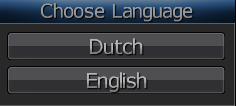
\includegraphics[width=0.4\linewidth]{../images/translation_manager_1}
\caption[]{Een Language Gui.}
\label{fig:trans1}
\end{figure}

Bij deze gui hoort de volgende code:

\begin{code}
class languageGui
{
private:
   GuiObjs obj;  
   Window * window;
   Button * buttonDutch;
   Button * buttonEnglish;
   
public:     
   void create()
   {
      obj.load(=== drop gui object here ===);
      window        = obj.findWindow("window"       );
      buttonDutch   = obj.findButton("buttonDutch"  );
      buttonEnglish = obj.findButton("buttonEnglish");
      
      Gui += obj;
   }
}
languageGui LanguageGui;
\end{code}

Vergeet niet de create functie uit de voeren in \eeFunc{Init()}.

Maak ook alvast een class \eeClass{translationManager}. Die ziet er voorlopig zo uit.

\begin{code}
class translationManager {
private:
	LANG_TYPE language = LANG_ENGLISH;

public:
	void setLanguage(LANG_TYPE language) {
		T.language = language;
	}	

	C Str & translate(C Str & text) {
		return text;
	}
}
translationManager TM;
\end{code}

In deze class kan je een ingestelde taal onthouden via de enum \eeClass{LANG\_TYPE}. Daarnaast zijn er functies om de taal in te stellen en een string te vertalen. Die laatste functie heeft voorlopig gewoon de input als resultaat. We werken deze class later verder uit, maar kunnen ze nu al gebruiken om de basis van het programma uit te werken.

Nu de translation class bestaat, kunnen we ook de Gui classes afwerken. In de class \eeClass{languageGui} zullen we callback functies voor de buttons schrijven:

\begin{code}
static void funcDutch(ptr)
{
  TM.setLanguage(LANG_DUTCH);
}

static void funcEnglish(ptr)
{
  TM.setLanguage(LANG_ENGLISH);
}
\end{code}

Vergeet niet deze functies aan de respectievelijke buttons te koppelen, en voeg daarna ook de volgende functie aan de class \eeClass{languageGui} toe:

\begin{code}
void translate()
{
  window       .setTitle(TM.translate("Choose Language"));
  buttonDutch  .setText (TM.translate("Dutch"          ));
  buttonEnglish.setText (TM.translate("English"        ));
}
\end{code}

De bovenstaande functie maakt al duidelijk hoe we tewerk zullen gaan. We gebruiken Engelse teksten om de content van de Gui elementen in te stellen. Maar die tekst wordt eerst door de translation manager gestuurd. Daar kunnen we dan als resultaat de vertaling geven.

\section{The translationManager Class}
Tijd om aan het echte werk te beginnen: de translation manager. Deze heeft een container nodig om vertaalde strings op te slaan. Maar een container is niet erg geschikt voor dit doel. 

Typisch voor deze class is dat we steeds een Engelse tekst hebben en die willen vervangen door een alternatief in een andere taal. In een taal zoals php zou je dat op de volgende manier doen:

\begin{code}
translations["Life"] = "Leven";
\end{code}

\ldots wat toelaat om achteraf de vertaling te bekomen via:
\begin{code}
void printText(string s) {
   echo translations[s];
}
\end{code}

Zoiets kan niet in C++. De index van een container moet steeds een integer zijn. Hoe pak je dat dan aan?

\section{Map}
De held van de dag is de class \eeClass{Map}. Een map is perfect voor waarden die via een \'e\'en op \'e\'en relatie met mekaar gelinkt zijn, zoals een vertaling. Waar we een \eeClass{Memc} defini\"eren met enkel zijn data type:

\begin{code}
Memc<Str> strings;
\end{code}

vermelden we in \eeClass{Map} ook het type van de index:

\begin{code}
Map<Str, Str> translations;
\end{code}

Het eerste argument noemen we KEY, het tweede DATA. Niet enkel strings kunnen een key zijn, maar om het even welke class. En dat schept een nieuw probleem: om effici\"ent te zoeken in een Map, moet die intern gesorteerd worden. En om dat te doen, moet \eeClass{Map} elementen kunnen vergelijken. \eeClass{Map} moet kunnen beslissen of een key groter, kleiner of gelijk is aan een andere key. 

Je zal zelf een functie moeten schrijven die elementen vergelijkt. De definitie van \eeClass{Map} toont je hoe. Als eerste argument van de constructor map staat er:

\begin{code}
Int compare(C KEY &a, C KEY &b)
\end{code}

Je moet dus een functie schrijven die twee argumenten van hetzelfde type als je key aanvaardt, en die een integer als resultaat heeft. Esenthel verwacht dat dat resultaat -1, 0 of 1 is. 

\begin{itemize}
	\item -1: het eerste argument is kleiner dan het tweede.
	\item  0: beide argumenten zijn gelijk.
	\item  1: het eerste argument is groter dan het tweede.
\end{itemize}

Aangezien we in deze map een key van het type \eeClass{Str} hebben, is de oplossing heel eenvoudig. Er bestaat namelijk al een functie om strings op deze manier met mekaar te vergelijken. We kunnen de gevraagde functie dus zo schrijven: 

\begin{code}
static int mapCompare(C Str &a, C Str &b)
{
  return CompareCI(a, b);
}
\end{code}

Indien je een verschil wil maken tussen hoofdletters en kleine letters, kan je ook \eeFunc{CompareCS} gebruiken.

\begin{note}
Merk op dat dit een static functie is, net zoals een callback die je aan een button doorgeeft.
\end{note}

Nu deze functie bestaat, kan je de definitie van je Map verbeteren:

\begin{code}
Map<Str, Str> textMap(mapCompare);
\end{code}

\section{Load a translation}
Nu de map bestaat, maken we een functie om een bestand te laden en de inhoud in de map op te slaan.

We kiezen er in dit voorbeeld voor om te werken met een tekstbestand. In dat bestand staat telkens een Engelse tekst, gevolgd door een vertaling. De tekst en de vertaling worden gescheiden door een dubbele punt:

\begin{code}
Choose Language: Kies je taal
Dutch: Nederlands
English: Engels
\end{code}

Je maakt nu in de class \eeClass{translationManager} de volgende functie:

\begin{code}
void loadLanguage() {
	textMap.clear();
	if(language == LANG_ENGLISH) return;
}
\end{code}

Daarmee wijs je bij het laden van een vertaling eerst de bestaande vertaling. Wanneer de nieuwe taal Engels is, dan stoppen we de functie omdat er geen vertaling nodig is.

In het andere geval moeten we een bestand laden. Dit bestand zou uit een config directory kunnen komen, maar in dit geval importeren de vertalingen in het project. Dat kan zo:

\begin{enumerate}
	\item Maak een bestand `dutch.txt' met de inhoud hierboven.
	\item Sleep het bestand in de editor.
	\item Sleep het bestand naar de read functie, zoals in de code hieronder.
\end{enumerate}

Voeg aan de bovenstaande functie de volgende code toe:
\begin{code}
FileText ft;
switch(language) {
	case LANG_DUTCH:
	{ 
	    ft.read(=== drop file here ===);
	    break; 
	}
}
\end{code}

Je kan voor elke vertaling een bestand en een case instructie toevoegen. De functie \eeFunc{read} zorgt er voor dat het object \eeClass{ft} de inhoud van het bestand bevat.

\begin{note}
Telkens je content toevoegt aan het oorspronkelijke bestand, kan je in de editor rechts klikken op het bestand en `Reload' kiezen.
\end{note}

Tot slot moet elke regel in dit bestand gelezen worden, waarbij we de inhoud toevoegen aan de \eeClass{Map}. We gebruiken daarbij een container `parts' en de functie \eeFunc{Split}. De Split functie verdeelt elke regel in twee delen en slaat die op in `parts'. Bijgevolg bevat \eeFunc{parts[0]} de key en \eeFunc{parts[1]} de data.

\begin{code}
while(!ft.end())
{
 	Str line = ft.getLine();
 	Mems<Str> parts;
 	Split(parts, line, ':');
 
	(*textMap.get(parts[0])) = parts[1];
}
\end{code}

In de laatste regel gebruiken we de \eeFunc{get} functie van \eeClass{Map}, met als eerste argument de key. Die key bestaat nog niet, dus \eeClass{Map} maakt een nieuw element aan. De data ken je toe aan dat element.

Nu is de nieuwe vertaling wel geladen, maar de Gui zal die niet vanzelf gebruiken. Wel hebben we in de gui class een functie translate voorzien. Het is dus nodig om na het laden van een vertaling alle Gui's te updaten. We maken daar een afzonderlijke functie voor:

\begin{code}
void updateGuis()
{
  StatsGui.translate();
  // add other Gui's that must be translated
}
\end{code}

En nu kan je de functie \eeFunc{setLanguage} vervolledigen:

\begin{code}
void setLanguage(LANG_TYPE language)
{
  T.language = language;
  loadLanguage();
  updateGuis();
}
\end{code}

Wat nu nog ontbreekt is de werkelijke vertaling. Je past de functie \eeFunc{translate} aan en voegt de volgende code toe:

\begin{code}
C Str & translate(C Str & text)
{
  Str * result = textMap.find(text));
  if(result != null) return *result;
  
  return text;
}
\end{code}





